% Finished August 17, 2012
% Split in half October 15, 2013.  (This is the second half.)
% Put into VUW thesis format (with Figure numbers) November 2013.

\documentclass[12pt, a4paper, twoside, openright]{book}

\usepackage{vuwthesis} % sets up some local things, mostly the front page

\setlength{\intextsep}{12pt} % set space above and below in-line float
\setlength{\abovecaptionskip}{0pt} % set space between figure and caption.


\usepackage{amssymb, amsmath}
\usepackage{tikz}

\author{Nat Lund}
\title{Chapter 2: Does Slip Exist?}

\newcommand{\beff}{\ensuremath{b_{\mathrm{eff}}}}

\newcommand{\ewf}{\ensuremath{\epsilon_{\mathrm{wf}}}}

\newcommand{\vslip}{\ensuremath{v_{\mathrm{slip}}}}

\newcommand{\paper}[1]
         {\colorbox[gray]{0.8}{ \textsc{#1}}
         
         }

\begin{document}
\chapter{Does Slip Exist? (Old)}

If the reader is confident that fluid slip exists, then this chapter may be skipped.  Alternatively, if the slip length is accepted as a being merely a parameter in a mathematical model, and only the mathematical solutions are of interest, then this chapter is superfluous.

However, practical applications of an effective slip length formula require some kind of slip effect to physically exist.  Establishing that a slip effect exists on clean, atomically flat surfaces is far from trivial.  Therefore, in this chapter we will dig quite deeply into the literature on the experimental and theoretical evidence for slip.

Any practical applications of the theory of effective slip length require that intrinsic slip effects are physically significant.  Establishing that a slip effect exists on clean, atomically flat surfaces is far from trivial.  Therefore, in this chapter we will examine into the literature on the experimental and theoretical evidence for slip.

%The work of this thesis is predicated on the existence of slip. Therefore, we will examine experimental and %theoretical evidence for slip in the literature.  
This cannot be a comprehensive review of all available literature, but rather will be a sample of some high-profile papers.
An exhaustive review of the experimental literature is available in the 2005 review article by Neto \emph{et al} \cite{NetoReview2005}. Other comprehensive reviews are by Vinogradova in 1999 \cite{VinogradovaReview1999} and Lauga, Brenner and Stone in 2006 \cite{LaugaReview2006}. A reasonable introduction is the progress article of Granick \emph{et al} from 2003 \cite{GranickReview2003}.

\section*{Types of Slip}

So far, we have discussed slip within a mathematical model of fluid flow; this is deliberate: in such a model the concepts of slip and slip length are straightforward and intuitive. However, we now need to tackle slip in the real world, disentangling a partially-ordered hierarchy of concepts.

\subsubsection*{Slip Effect}

We begin by considering the concept of a most general slip \emph{effect.} A surface may be described as exhibiting slip if it behaves \emph{as if} fluid slipped on the surface.  For example, for a given pressure, a tube may flow liquid at a rate \emph{as if} it were slightly wider; hence, we could consider it to have a non-zero slip length. But this says nothing about the real conditions on the fluid-solid boundary in the tube. We simply don't know what the fluid velocity at the boundary is. It is possible that the boundary velocity is non-zero, or there may be other effects causing the increased flow. All we can say is that there is a `slip effect'.

\subsubsection*{Intrinsic Slip}

Next, we turn our attention to the \emph{material} of the surface exhibiting  slip effect. Suppose we can prepare a perfectly clean, atomically flat sample of the material. Further, suppose we can experimentally test the sample for slip effects with some pure liquid (pure water, say). If the slip effect still appears, and is replicable, then the implied slip length is a meaningful, reliable parameter of the fluid/solid system. It is reasonable to label this the \emph{intrinsic} slip length.

\subsubsection*{Molecular Slip}

Thus, in the foregoing, slip length is \emph{imputed} to the surface: we \emph{regard} the surface as having a slip length. What would it mean to \emph{really} have a finite slip length? To say anything about the velocity at the surface, we must assume that velocity is well defined. The soothing infinitely-divisible continuum of our model must be replaced with a statistical mechanical definition: the average velocity of some suitable ensemble of \emph{molecules.} Hence, `true' slip entails fluid molecules in some sense sliding over solid molecules. Start by considering a molecule incident on a surface: it has some velocity in the direction tangential to the surface; likewise if it leaves the surface. It is easier to first consider the condition of no slip, then relax that condition. No slip suggests that fluid molecules \emph{stick} to the surface, and if they release, they leave at a \emph{random} angle to the surface, so that the \emph{average} tangential velocity of detaching molecules is the same as the velocity of the surface. Slip suggests, then, that molecules leave the surface with a tangential velocity that \emph{correlates} with the tangential velocity at which they impacted. (Perfect correlation is of course specular reflection --- corresponding to perfect slip, or infinite slip length.) A sensible term for this phenomenom is \emph{molecular slip.}

\subsubsection*{Apparent Slip}

While slip effects are generally acknowledged, the existence of molecular slip remains debatable. Perhaps the simplest alternative to molecular slip to explain slip effects is apparent slip. The idea is that there exists a \emph{boundary layer} of reduced viscosity at the solid surface. As a consequence of the lower viscosity, the velocity gradient in the boundary layer is \emph{steeper} than in the bulk. Thus, the velocity gradient `turns a corner' at the interface between boundary layer and bulk. The no-slip condition holds at the solid/liquid interface, but the velocity gradient in the bulk can be extrapolated to generate a slip length.  A schematic illustrating this appears in Figure (\ref{depletion}).

The boundary is very thin compared to experimental length scales. The reduction in viscosity is commensurate with a reduction in density; indeed, de Gennes notes that observed slip effects are explainable by a \emph{gas} layer, only 1 or 2 atoms thick. 

\begin{figure}[ht]
\centering
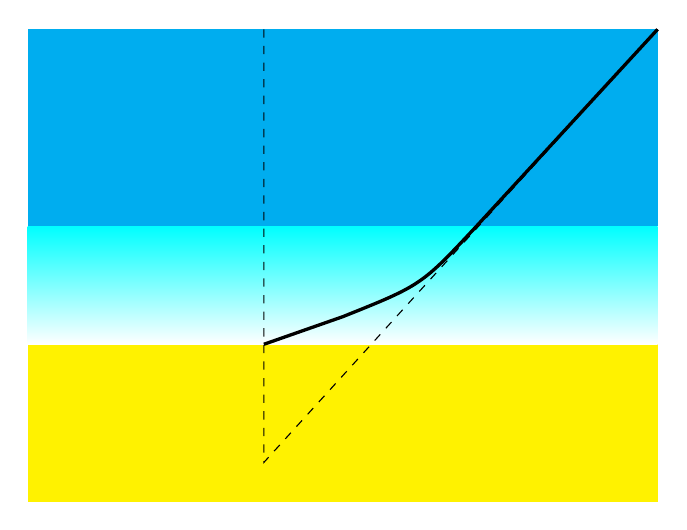
\begin{tikzpicture}

\fill[color=yellow] (-3,-2) rectangle (5,0);

\fill[color=cyan] (-3,1.5) rectangle (5,4);
\shade [top color=cyan] (-3,0) rectangle (5,1.5);

\draw[dashed] (0,4) -- (0,-1.5) -- (5,4);

\draw[very thick] (0,0)--(1.0,0.35) .. controls (2, 0.75) .. (2.7,1.5)--(5,4);

\end{tikzpicture}
\caption{Apparent slip caused by a depletion layer with lower-than-bulk viscosity.} \label{depletion}
\end{figure}

\subsubsection*{Effective Slip}

Coming full circle back to a general slip effect, suppose we \emph{know} that the surface under test is not a pure surface.  Then we do not consider the implied slip length to be intrinsic. Instead, we label this the \emph{effective} slip length. This is Nature's average of the intrinsic slip lengths of the system.


\subsubsection*{Measured Slip}

Finally, as we shall see shortly, all measurements are to some extent indirect: Experiments cannot yet directly probe the fluid velocity in the region within a few nanometers of the surface. A measurement of a slip effect may be measuring molecular slip, apparent slip, or, for a heterogeneous surface, any combination of the two.


\clearpage
\subsection*{Definitions in the Literature}

The 2006 review article by Lauga, Brenner and Stone \cite{LaugaReview2006} proposes the following definitions (some paraphrased):

\begin{itemize}

\item \textbf{Phenomenon of slip:} A fluid dynamics system behaving as if the fluid velocity at the wall differs from the wall velocity.

\item \textbf{Molecular slip} (also intrinsic slip): `Refers to the possibility of using hydrodynamics to force liquid molecules to slip against solid molecules.'

\item \textbf{Apparent slip:} The case when the no-slip condition holds on the surface, but at larger length scales, the no-slip condition appears not to be valid.

\item \textbf{Effective slip:} `Refers to the case where molecular or apparent slip is estimated by averaging an appropriate measurement over the length scale of an experimental apparatus.'

\end{itemize}

It may not be immediately clear whether these definitions are compatible with ours, or not. The relationship is clarified once we note that the Lauga \emph{et al} definitions implicitly assume a \emph{homogeneous} surface. Therefore, they define effective slip to be an indirectly measured slip length of a pure surface. The measured slip must then be due to either molecular slip or apparent slip.

By contrast, we explicitly allow a mixed-slip surface. Thus, a measured slip length may be either 1) an effective slip length, or 2) an intrinsic slip length, if we are confident that the surface is pure and uncontaminated. Thus, we redefine effective slip for use on mixed-slip surfaces, and redefine intrinsic slip as pertaining to surfaces that we \emph{know} to be homogeneous.
Hence, the Lauga \emph{et al} use of the phrase `effective slip' falls under our definition of the indirectly measured slip length of a homogeneous surface --- that is, our definition of intrinsic slip. Obviously, we now distinguish between intrinsic and molecular slip. Our definitions of molecular slip are the same.

%%%%%%%%%%%%%%%%%%%%%%%%%%%%%%%%%%%%%%%%%%%%%%%%%%%%%%%%%%%%%%%%%%%%%%%%%%%%%%%%
%%%%%%%%%%%%%%%%%%%%%%%%%%%%%%%%%%%%%%%%%%%%%%%%%%%%%%%%%%%%%%%%%%%%%%%%%%%%%%%%

\chapter{Does Slip Exist?}

%If the reader is confident that fluid slip exists, then this chapter may be skipped.  Alternatively, if the slip length is accepted as a being merely a parameter in a mathematical model, and only the mathematical solutions are of interest, then this chapter is superfluous.

%However, practical applications of an effective slip length formula require some kind of slip effect to physically exist.  Establishing that a slip effect exists on clean, atomically flat surfaces is far from trivial.  Therefore, in this chapter we will dig quite deeply into the literature on the experimental and theoretical evidence for slip.

%Any practical applications of the theory of effective slip length require that intrinsic slip effects are physically significant.  Establishing that a slip effect exists on clean, atomically flat surfaces is far from trivial.  Therefore, in this chapter we will examine into the literature on the experimental and theoretical evidence for slip.

A theory of effective slip could be treated as a purely mathematical result, with the slip length being just a parameter in the model.  However, such a theory has practical applications only if the slip length has some physical meaning: quantifying the slip effect for flow over a homogeneous surface.  Establishing that a slip effect exists on clean, atomically flat surfaces is far from trivial.  Therefore, in this chapter we will examine the literature on the experimental and theoretical evidence for slip.

This cannot be a comprehensive review of all available literature, but rather will be a sample of some high-profile papers.
An exhaustive review of the experimental literature is available in the 2005 review article by Neto \emph{et al} \cite{NetoReview2005}. Other comprehensive reviews are by Vinogradova in 1999 \cite{VinogradovaReview1999} and Lauga, Brenner and Stone in 2006 \cite{LaugaReview2006}. A reasonable introduction is the progress article of Granick \emph{et al} from 2003 \cite{GranickReview2003}.

\section*{Types of Slip}

So far, we have discussed slip within a mathematical model of fluid flow; this is deliberate: in such a model the concepts of slip and slip length are straightforward and intuitive. However, we now need to tackle slip in the real world, disentangling a partially-ordered hierarchy of concepts.

\clearpage
\subsection*{Definitions in the Literature}

The 2006 review article by Lauga, Brenner and Stone \cite{LaugaReview2006} proposes the following definitions (some paraphrased):

\begin{itemize}

\item \textbf{Phenomenon of slip:} A fluid dynamics system behaving as if the fluid velocity at the wall differs from the wall velocity.

\item \textbf{Molecular slip} (also intrinsic slip): `Refers to the possibility of using hydrodynamics to force liquid molecules to slip against solid molecules.'

\item \textbf{Apparent slip:} The case when the no-slip condition holds on the surface, but at larger length scales, the no-slip condition appears not to be valid.

\item \textbf{Effective slip:} `Refers to the case where molecular or apparent slip is estimated by averaging an appropriate measurement over the length scale of an experimental apparatus.'

\end{itemize}


These definitions are a good place to start.  But they make no mention of \emph{mixed-slip} surfaces.  We shall accept these definitions, but modify and extend them to deal cleanly with the separate cases of pure \emph{and} mixed-slip surfaces.

The first modification is to separate molecular slip from intrinsic slip.

\begin{itemize}
\item \textbf{Intrinsic Slip:} When a clean, atomically flat homogeneous surface behaves as if the no-slip condition does not hold.
\end{itemize}

With this definition, Intrinsic Slip may be due to Molecular Slip or Apparent Slip.

The second modification is to take Lauga \emph{et al}'s concept of `Effective Slip' and simplify it, then relabel it as simply `Measured Slip'.

\begin{itemize}
\item \textbf{Measured Slip:} A slip effect measured with some experimental apparatus.
\end{itemize}

This allows us to use the phrase `Effective Slip' to emphasize the possible heterogeneity of the surface:

\begin{itemize}
\item \textbf{Effective Slip:} A slip effect imputed to liquid-solid interface, where the surface is not known to be homogeneous and atomically flat.
\end{itemize} 

We shall discuss some of these concepts in more depth.

\subsubsection*{Measured Slip}
As we shall see shortly, all measurements are to some extent indirect: Experiments cannot yet directly probe the fluid velocity in the region within a few nanometers of the surface. A measurement of a slip effect may be measuring molecular slip, apparent slip, or, for a heterogeneous surface, any combination of the two.

There are no direct measurements of slip; if there were, they would be measuring molecular slip.


\subsubsection*{Intrinsic Slip}
%Next, we turn our attention to the \emph{material} of the surface exhibiting  slip effect. 
Suppose we can prepare a perfectly clean, atomically flat sample of some material. Further, suppose we can experimentally test the sample for slip effects with some pure liquid.
% (pure water, say). 
If a slip effect appears, and can be consistently replicated, then the implied slip length is a meaningful, reliable parameter of the fluid-solid system. It is reasonable to label this the \emph{intrinsic} slip length.

Intrinsic slip may be due to molecular slip or apparent slip.


\subsubsection*{Molecular Slip}
`True slip' means that the fluid \emph{at the boundary} has a non-zero velocity.
At the smallest scale, the fluid velocity at a point is the average velocity of an ensemble of molecules.  Thus, `true' slip means that the average velocity of the molecules in contact with the wall is non-zero.
This implies that the molecules in contact with the wall are \emph{not} all sticking to the wall all the time.
If (some) fluid molecules at the surface are slipping along the surface, this is termed molecular slip.

There are no direct observations of molecular slip, though (as explained later) it is observed in molecular dynamics computer simulations.

A hypothetical mechanism for molecular slip in liquids could be one similar to the (known) mechanism for slip in gases -- Knudsen Slip:


\subsubsection*{$\bullet$ Slip in Gases -- Knudsen Slip}
In a gas, the mean free path is many times larger than the gas molecule size, so an interaction with the wall will almost certainly not involve another gas particle.  Therefore, the interaction can be treated as a simple reflection.

A gas particle incident on the wall has some momentum in the tangential direction.  If the particle bounces off the wall in specular reflection, then the tangential momentum does not change.  With no momentum loss, there is no `friction', and so the gas experiences perfect slip.  

At the other extreme, if an incident gas particle \emph{sticks} to the wall,
then all tangential momentum is transferred to the wall.  If the particle detaches with a velocity in a random direction, the \emph{average} tangential momentum will be zero -- the same as the wall.  This is the case of `stick', or the no-slip condition.

An analogous effect may occur in fluids, although the mean free path in a liquid is generally less than the molecular diameter, so angles of incidence and reflection become difficult to define.

\subsubsection*{Apparent Slip}

%While slip effects are generally acknowledged, the existence of molecular slip remains debatable. 
Perhaps the simplest alternative to molecular slip to explain slip effects is apparent slip. The idea is that there exists a \emph{boundary layer} of reduced viscosity at the solid surface. As a consequence of the lower viscosity, the velocity gradient in the boundary layer is \emph{steeper} than in the bulk. Thus, the velocity gradient `turns a corner' at the interface between boundary layer and bulk. The no-slip condition holds at the solid-liquid interface, but the velocity gradient in the bulk can be extrapolated to generate a slip length, as shown in Figure (\ref{depletion}).

\begin{figure}[ht]
\centering
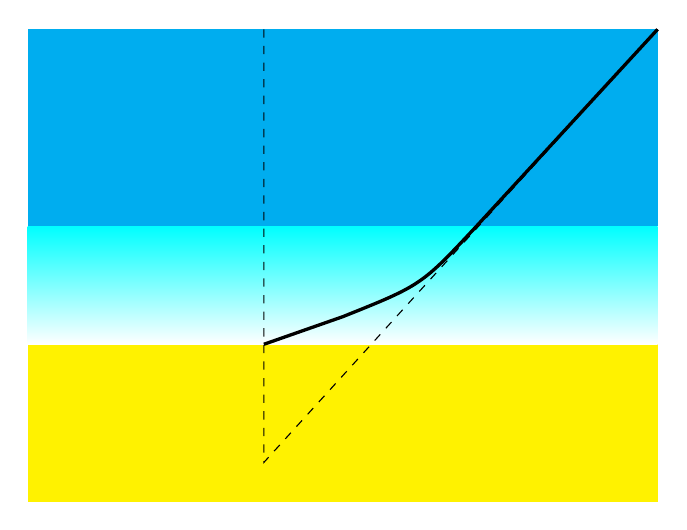
\begin{tikzpicture}

\fill[color=yellow] (-3,-2) rectangle (5,0);

\fill[color=cyan] (-3,1.5) rectangle (5,4);
\shade [top color=cyan] (-3,0) rectangle (5,1.5);

\draw[dashed] (0,4) -- (0,-1.5) -- (5,4);

\draw[very thick] (0,0)--(1.0,0.35) .. controls (2, 0.75) .. (2.7,1.5)--(5,4);

\end{tikzpicture}
\caption{Apparent slip caused by a depletion layer with lower-than-bulk viscosity.} \label{depletion}
\end{figure}

The boundary is very thin compared to experimental length scales. The reduction in viscosity is commensurate with a reduction in density; indeed, de Gennes notes that observed slip effects are explainable by a \emph{gas} layer, only 1 or 2 atoms thick \cite{deGennes2002}.

\clearpage
\subsection*{Types of Slip Redux}

We summarize the hierarchy of slip concepts in Figure (\ref{slipconcepts}) below:

\begin{figure}[ht]
\centering
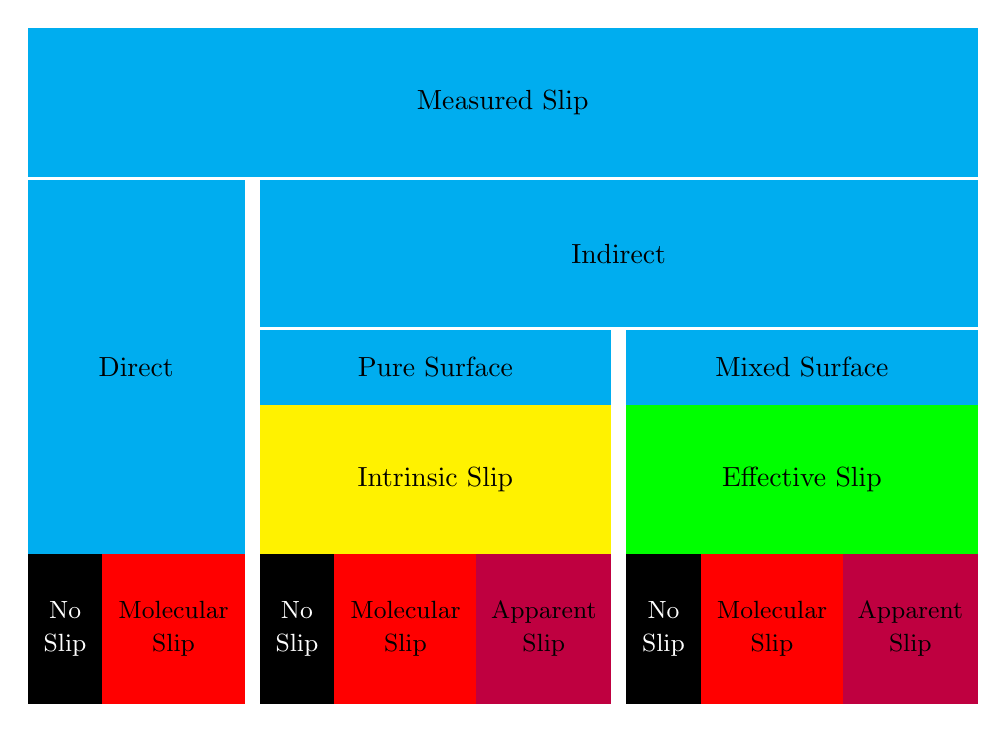
\begin{tikzpicture} [scale=0.95]
\renewcommand{\baselinestretch}{1.00}
% Depending on some random factors, the rectangles may appear on screen to have faint white
% borders between them, or not.  The slight separation is good.  So I have made this explicit
% by lifting the bottom of Measured Slip and Indirect rectangles by 0.04 cm 

\fill[color=black] (0,0) rectangle node[color=white,align=center] 
{\small No\\ \small Slip} +(1,-2);
\fill[color=red] (1,0) rectangle node[color=black,align=center] 
{\small Molecular\\ \small Slip} +(1.9,-2);

\fill[color=black] (3.1,0) rectangle node[color=white,align=center] 
{\small No\\ \small Slip} +(1,-2);
\fill[color=red] (4.1,0) rectangle node[color=black,align=center] 
{\small Molecular\\ \small Slip} +(1.9,-2);
\fill[color=purple] (6,0) rectangle node[color=black,align=center]
{\small Apparent\\ \small Slip} +(1.8,-2);

\fill[color=black] (8,0) rectangle node[color=white,align=center] 
{\small No\\ \small Slip} +(1,-2);
\fill[color=red] (9,0) rectangle node[color=black,align=center] 
{\small Molecular\\ \small Slip} +(1.9,-2);
\fill[color=purple] (10.9,0) rectangle node[color=black,align=center]
{\small Apparent\\ \small Slip} +(1.8,-2);

\fill[color=cyan] (0,0) rectangle node[color=black] {Direct} +(2.9,5);
\fill[color=cyan] (0,5.04) rectangle node[color=black] {Measured Slip} +(12.7,2);

\fill[color=yellow] (3.1,0) rectangle node[color=black] {Intrinsic Slip} +(4.7,2);
\fill[color=cyan] (3.1,2) rectangle node[color=black] {Pure Surface} +(4.7,1);

\fill[color=green] (8,0) rectangle node[color=black] {Effective Slip} +(4.7,2);
\fill[color=cyan] (8,2) rectangle node[color=black] {Mixed Surface} +(4.7,1);

\fill[color=cyan] (3.1,3.04) rectangle node[color=black] {Indirect} +(9.6,1.96);

\end{tikzpicture}
\caption{Hierarchy of slip concepts.} \label{slipconcepts}
\end{figure}

Note that the `Direct Measurement' category is there just for completeness --- experiments cannot presently verify molecular slip.


\bibliography{Lund_Thesis.bib}
\bibliographystyle{plain}

\end{document}
